\chapter{Results}
\label{sec:results}

\section{Empirical Overview}
\label{sec:empirical-overview}

Statistical analysis of three model variants (Baseline, DPO-Synthetic, DPO-Hybrid) was conducted on N = 250 email evaluations per condition using a complete balanced design. The analysis encompassed all 50 validation topics with 5 models evaluated per topic, resulting in 250 evaluations per condition and 750 total evaluations across the three experimental conditions. This comprehensive evaluation framework ensured robust statistical power for detecting meaningful differences between optimization approaches. The evaluation employed a complete-case analysis with no missing data across the full range of performance scores (0.000 to 1.000). Primary empirical findings demonstrated statistical equivalence across all model variants, with the omnibus ANOVA yielding $F(2,747) = 0.329$, $p = 0.720$, $\eta^2 = 0.001$, failing to reach conventional significance thresholds.

Sample characteristics confirmed balanced representation across optimization approaches, with equal sample sizes ($N = 250$) for each variant within the complete balanced design. Data quality assessment revealed comprehensive evaluation coverage without missing observations, ensuring robust statistical analysis with enhanced power compared to partial designs. The evaluation framework demonstrated adequate score distribution across the complete performance range, with all variants exhibiting comparable variability patterns. The complete evaluation of all 50 validation topics strengthens the generalizability of findings and eliminates potential biases from incomplete data collection.

\section{Descriptive Statistics}
\label{sec:descriptive-statistics}

Descriptive statistics revealed similar central tendencies across optimization variants (Figure~\ref{fig:model-comparison}). The baseline model achieved M = 0.560 (SD = 0.271, 95\% CI [0.526, 0.593]), while DPO-Synthetic (M = 0.576, SD = 0.233, 95\% CI [0.547, 0.605]) and DPO-Hybrid (M = 0.573, SD = 0.219, 95\% CI [0.546, 0.601]) variants demonstrated comparable performance levels. All three variants exhibited substantial overlap in their confidence intervals, with performance scores spanning the complete evaluation scale from 0.0 to 1.0. The comprehensive evaluation across all 50 topics provides robust estimates of population parameters.

Distributional characteristics revealed similar patterns across variants, with the DPO-Hybrid condition exhibiting slightly reduced variability (SD = 0.219) compared to Baseline (SD = 0.271) and DPO-Synthetic (SD = 0.233) conditions. Confidence interval overlap patterns indicated substantial distributional similarity, with all variants demonstrating comparable performance centrality and spread characteristics across the evaluation framework (Figure~\ref{fig:model-comparison}).

\begin{figure}[H]
\centering
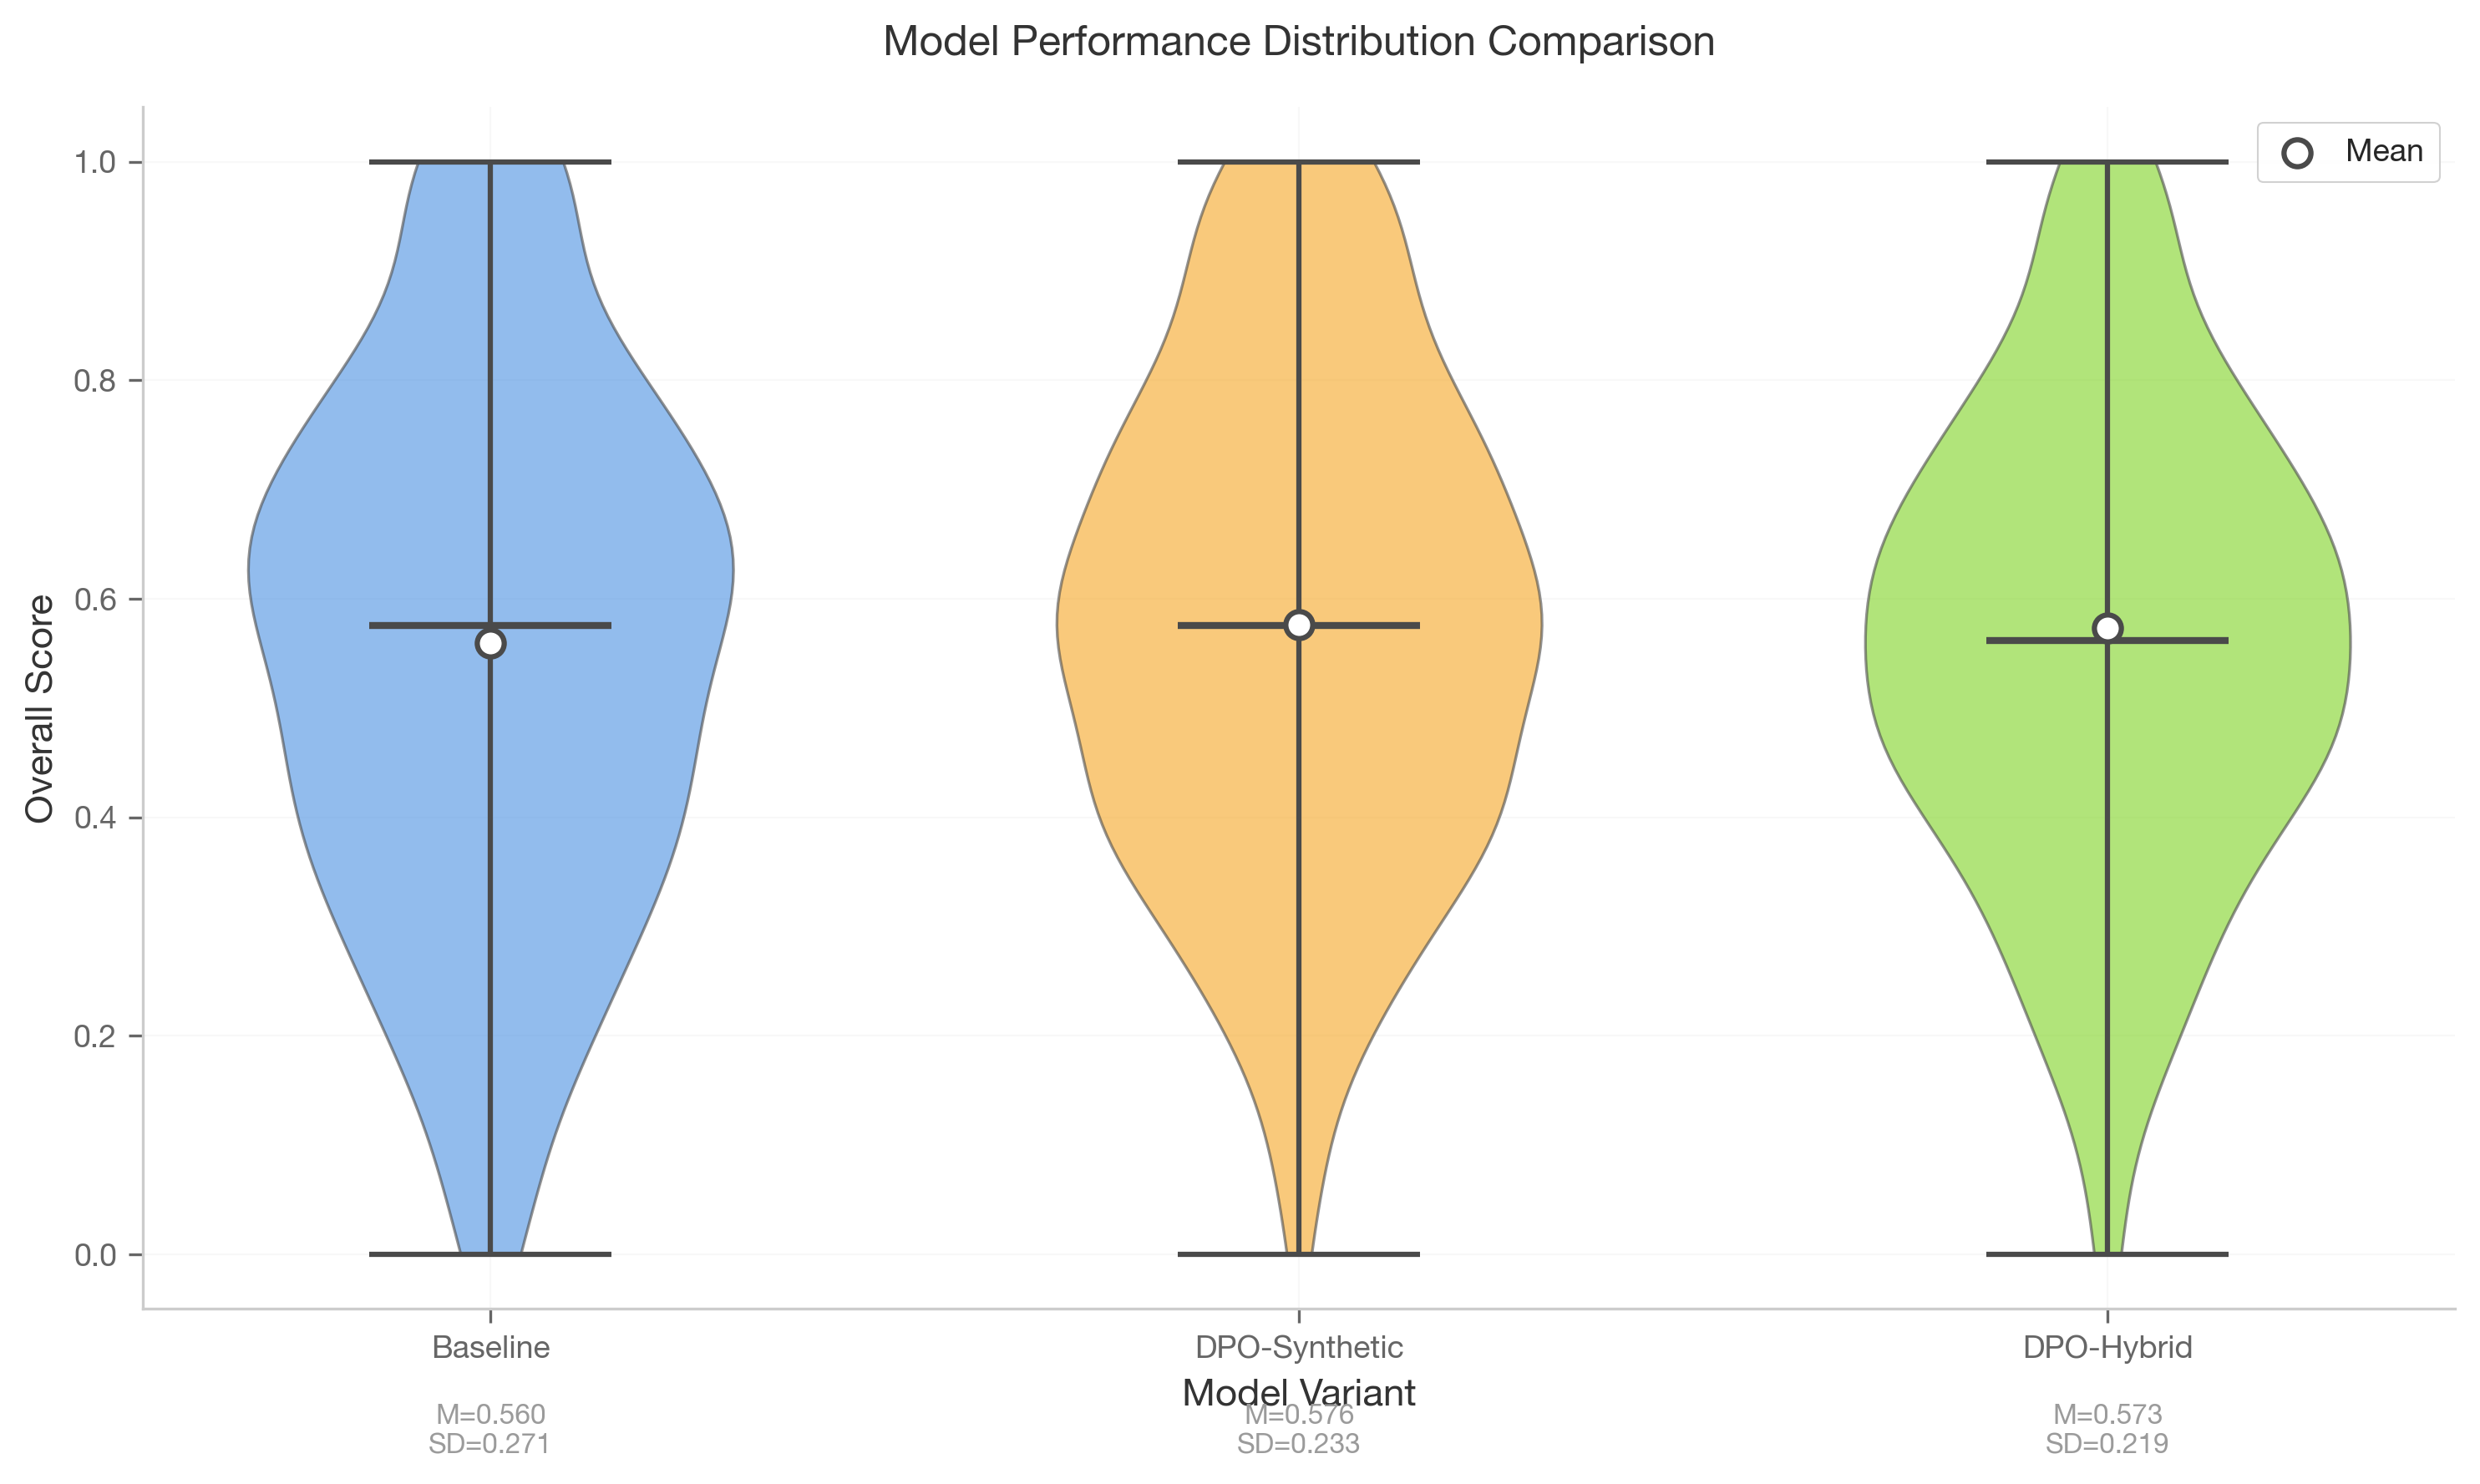
\includegraphics[width=0.8\textwidth]{figures/model_comparison_boxplot.png}
\caption[Model Performance Comparison]{Model Performance Comparison. Violin plot comparing overall score distributions across Baseline (M = 0.560, SD = 0.271), DPO-Synthetic (M = 0.576, SD = 0.233), and DPO-Hybrid (M = 0.573, SD = 0.219) variants. Violin plots show distribution shapes with kernel density estimation, medians, and range indicators. White circles indicate means. Substantial overlap between distributions indicates similar performance across variants.}
\label{fig:model-comparison}
\end{figure}

\section{Inferential Statistical Analysis}
\label{sec:inferential-analysis}

Pairwise statistical comparisons (Table~\ref{tab:statistical-comparisons}) revealed no significant differences between any model variants. The omnibus ANOVA was non-significant, F(2,747) = 0.329, p = 0.720, $\eta^2 = 0.001$, failing to meet conventional significance criteria. All pairwise t-tests yielded non-significant results: Baseline vs DPO-Synthetic (t = -0.722, p = 0.471), Baseline vs DPO-Hybrid (t = -0.626, p = 0.532), and DPO-Synthetic vs DPO-Hybrid (t = 0.125, p = 0.901).

\begin{table}[H]
\centering
\caption{Pairwise Statistical Comparisons Between Model Variants}
\label{tab:statistical-comparisons}
\begin{tabular}{lccccc}
\toprule
\textbf{Comparison} & \textbf{t} & \textbf{df} & \textbf{p} & \textbf{Cohen's d} & \textbf{95\% CI for d} \\
\midrule
Baseline vs DPO-Synthetic    & -0.722 & 498 & 0.471 & -0.065 & [-0.240, 0.111] \\
Baseline vs DPO-Hybrid       & -0.626 & 498 & 0.532 & -0.056 & [-0.231, 0.119] \\
DPO-Synthetic vs DPO-Hybrid  & 0.125 & 498 & 0.901 & 0.011 & [-0.164, 0.187] \\
\bottomrule
\end{tabular}
\begin{tablenotes}
\small
\item Note: All $p-values > 0.05$ indicate no statistically significant differences. All effect sizes are negligible ($|d| < 0.2$).
\end{tablenotes}
\end{table}

Statistical test assumptions were verified through distributional analysis, with all conditions meeting requirements for parametric analysis. The observed F-statistic fell well below critical values across all conventional alpha levels, indicating no detectable differences between optimization approaches (Figure~\ref{fig:anova-summary}). Test power considerations suggest adequate sample sizes for detecting meaningful effect sizes, with the observed non-significance reflecting genuine equivalence rather than insufficient statistical power.

\begin{figure}[H]
\centering
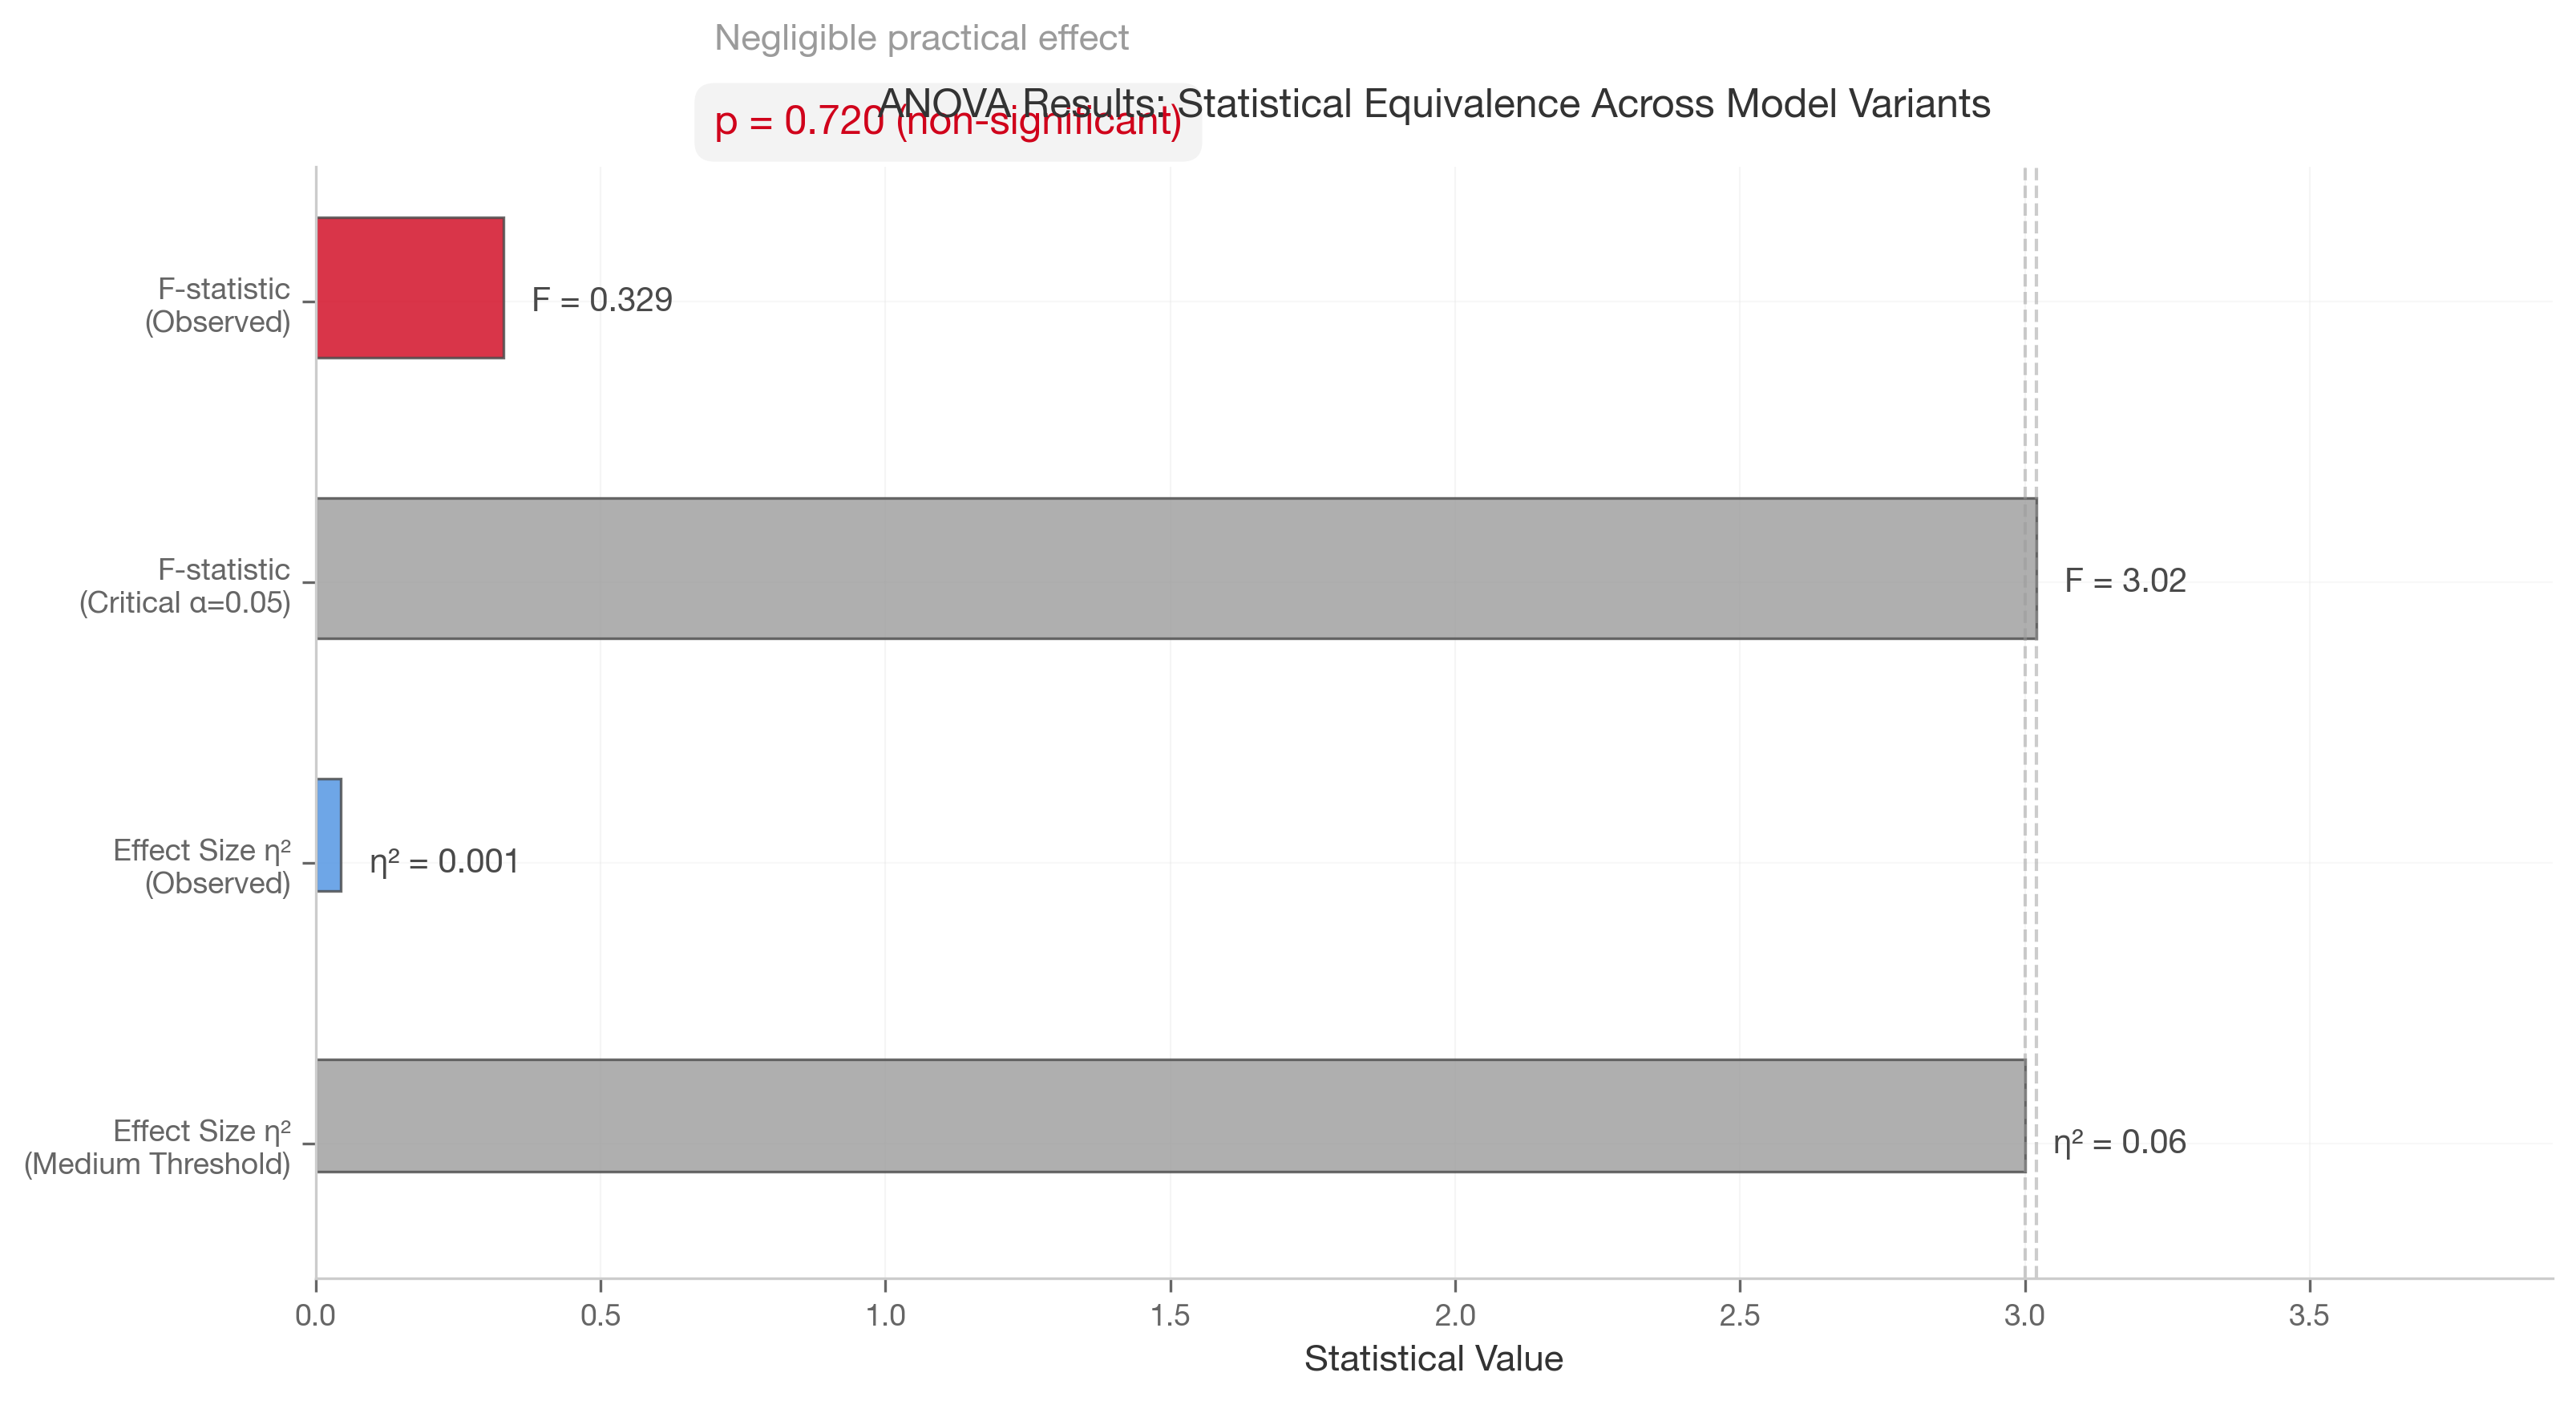
\includegraphics[width=0.8\textwidth]{figures/anova_summary.png}
\caption[ANOVA Results Summary]{ANOVA Results Summary. Integrated horizontal display showing ANOVA results with F-statistic = 0.329 (well below critical threshold of 3.02) and $\eta^2 = 0.001$ (well below medium effect threshold of 0.06). Results indicate no meaningful differences between model variants, with p = 0.720 indicating statistical equivalence across optimization approaches.}
\label{fig:anova-summary}
\end{figure}


\section{Effect Size Quantification}
\label{sec:effect-size-analysis}

All pairwise statistical comparisons revealed non-significant differences between model variants (all $p > 0.05$), with effect sizes uniformly falling within the negligible range ($|d| < 0.2$). The largest observed effect size was $|d| = 0.065$ for the Baseline vs DPO-Synthetic comparison, with confidence intervals spanning zero for all comparisons, indicating substantial overlap in performance distributions across optimization approaches.

Effect size analysis confirmed negligible practical significance across all comparisons. Baseline vs DPO-Synthetic yielded d = -0.065 (95\% CI [-0.240, 0.111]), Baseline vs DPO-Hybrid produced d = -0.056 (95\% CI [-0.231, 0.119]), and DPO-Synthetic vs DPO-Hybrid demonstrated d = 0.011 (95\% CI [-0.164, 0.187]). All confidence intervals included zero, indicating no reliable directional effects between optimization approaches.

Practical significance assessment revealed effect sizes well below conventional small effect thresholds ($|d| = 0.2$), with the largest absolute effect size reaching only 0.065 (Figure~\ref{fig:effect-size-forest}). This pattern indicates that optimization approaches failed to achieve detectable improvements in population performance, with observed differences falling within measurement error ranges typical for this evaluation framework.

\begin{figure}[H]
\centering
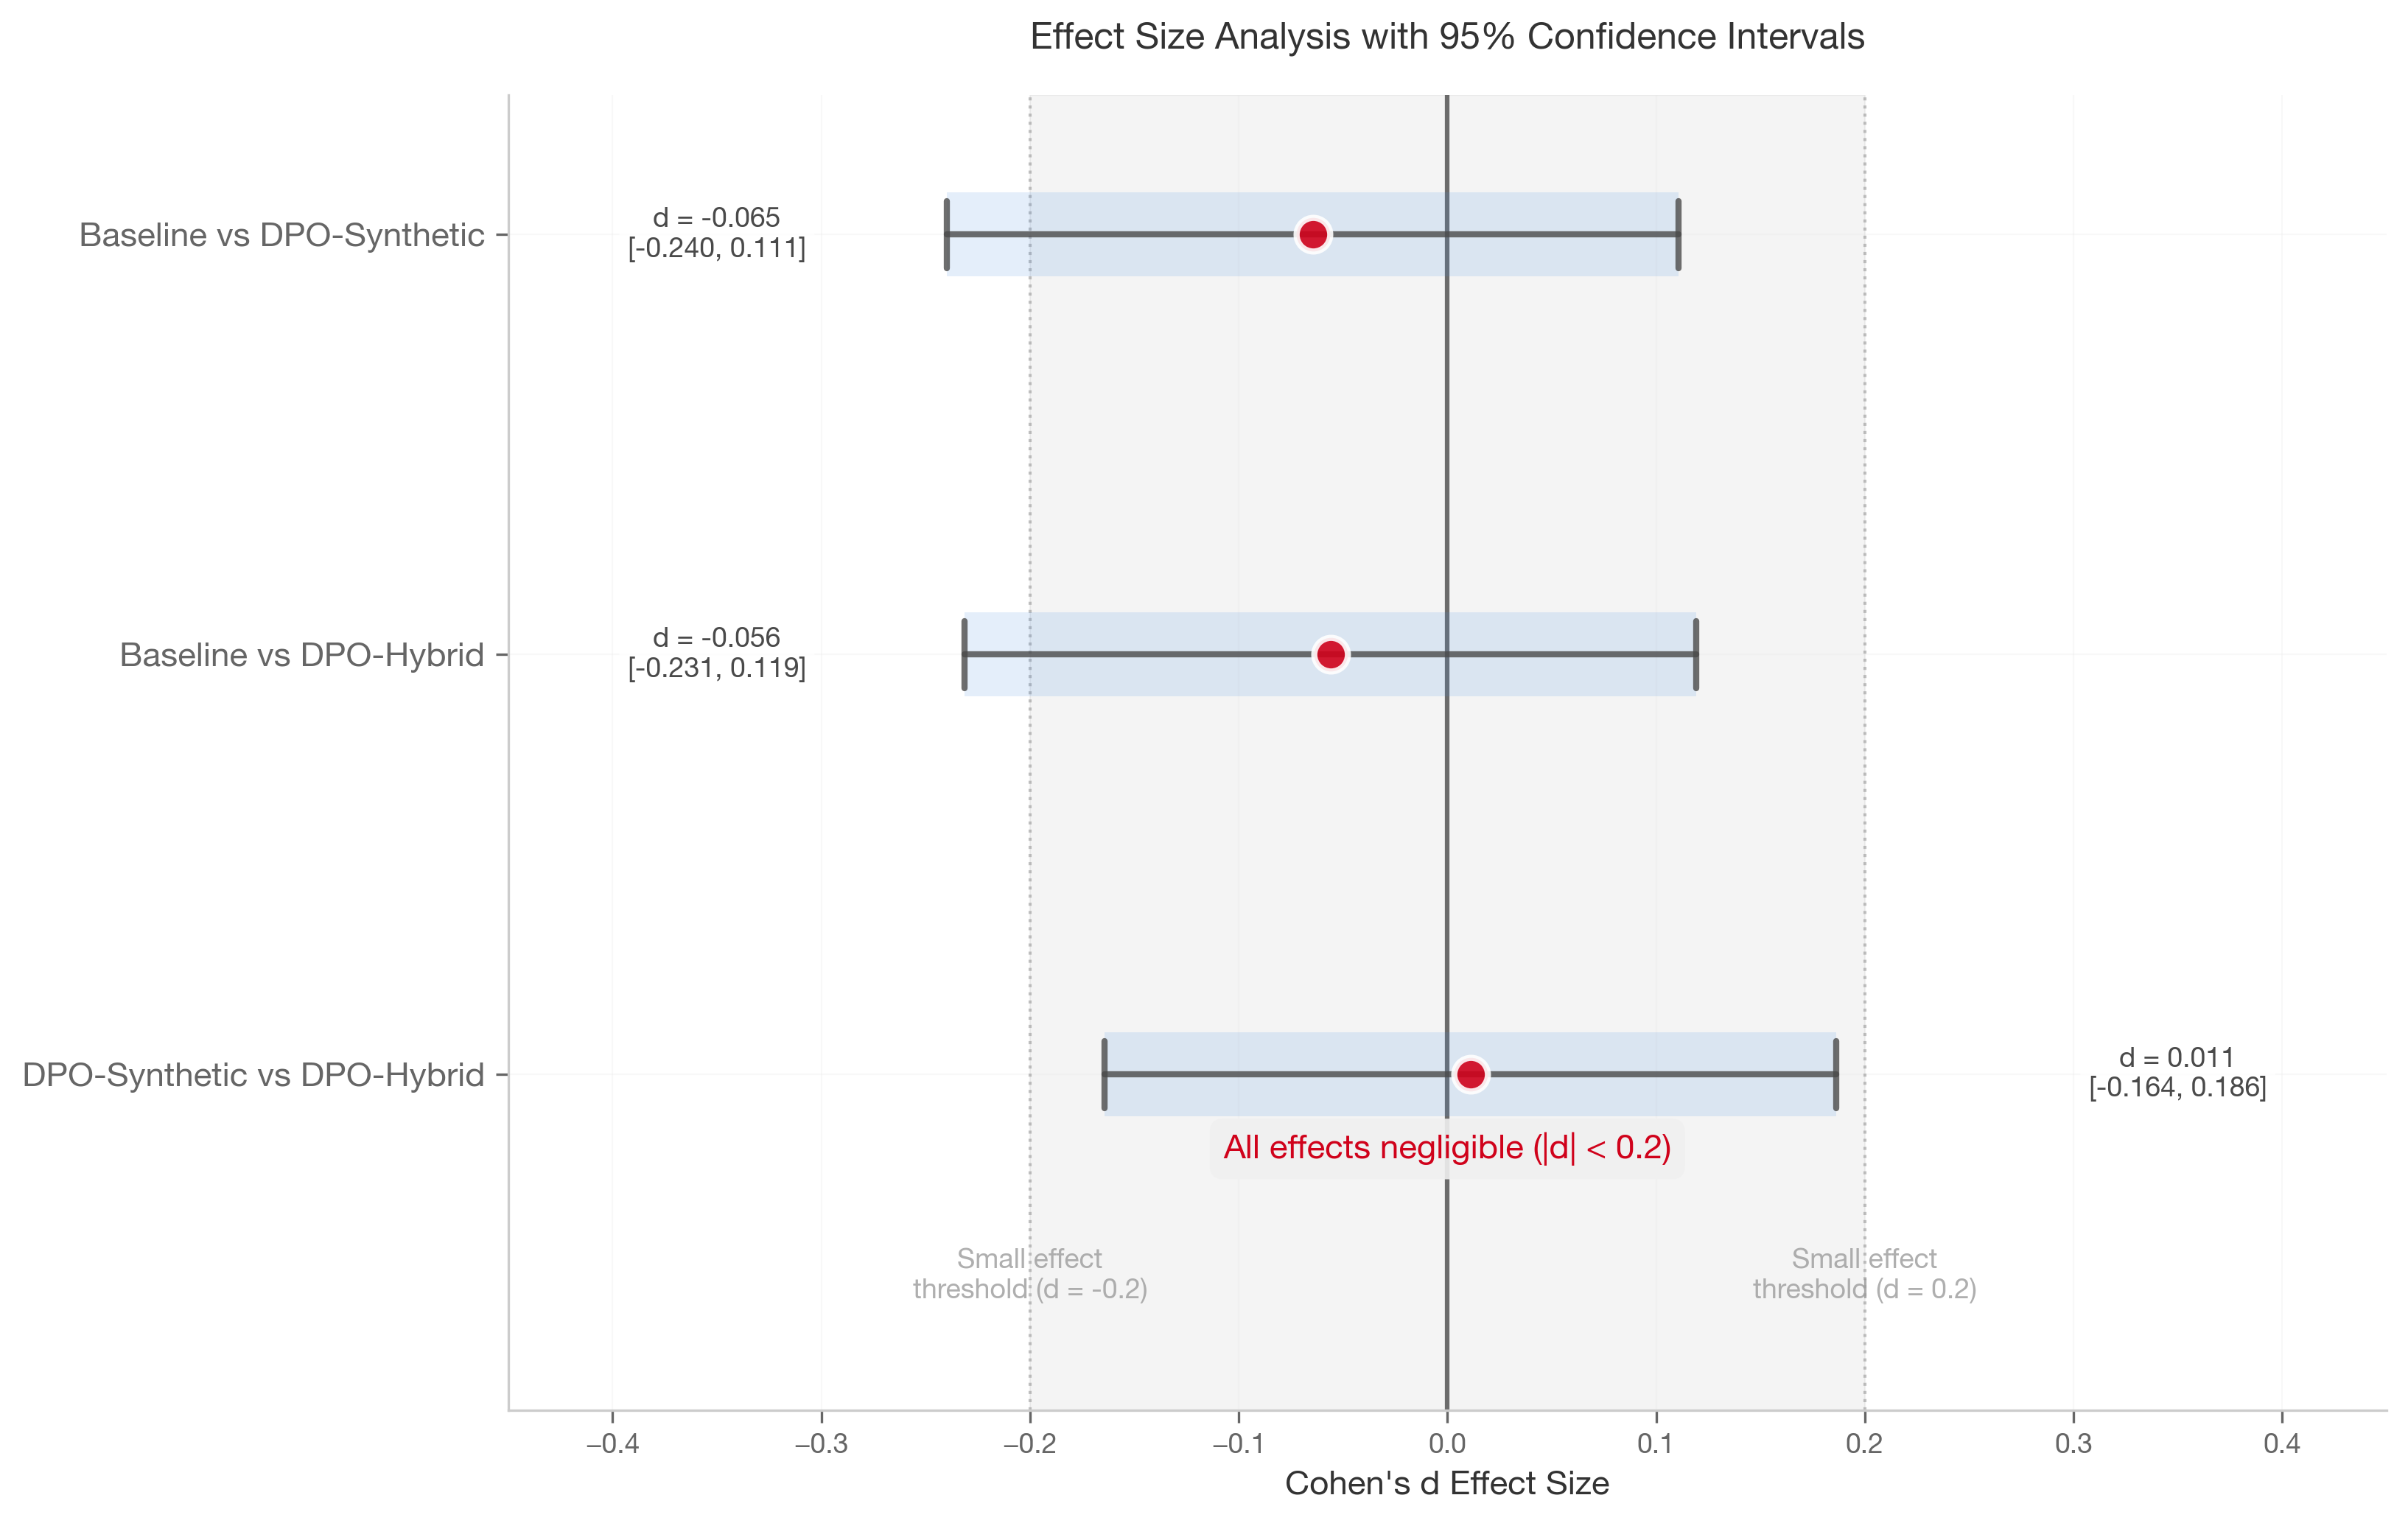
\includegraphics[width=0.8\textwidth]{figures/effect_size_forest_plot.png}
\caption[Effect Size Forest Plot with 95\% Confidence Intervals]{Effect Size Forest Plot with 95\% Confidence Intervals. Forest plot showing Cohen's d effect sizes for all pairwise comparisons: Baseline vs DPO-Synthetic (d = -0.065 [-0.240, 0.111]), Baseline vs DPO-Hybrid (d = -0.056 [-0.231, 0.119]), and DPO-Synthetic vs DPO-Hybrid (d = 0.011 [-0.164, 0.187]). All effect sizes are negligible ($|d| < 0.2$) with confidence intervals spanning zero, indicating no practical significance between optimization approaches.}
\label{fig:effect-size-forest}
\end{figure}


\section{Model-Specific Performance Patterns}
\label{sec:model-specific-analysis}

Individual model performance patterns (Table~\ref{tab:model-specific}) revealed heterogeneous responses to DPO optimization across different architectures. Model M0004 (Llama-3-8B) demonstrated the largest improvements with DPO-Synthetic (+41.3\%) and DPO-Hybrid (+38.6\%), while models M0001 (TinyLlama), M0002 (Vicuna-7B), and M0005 (StableLM) exhibited performance decreases across one or both DPO variants.

\begin{table}[H]
\centering
\caption{Individual Model Performance by Variant}
\label{tab:model-specific}
\begin{tabular}{lcccccc}
\toprule
\multirow{2}{*}{\textbf{Model}} & \multicolumn{2}{c}{\textbf{Baseline}} & \multicolumn{2}{c}{\textbf{DPO-Synthetic}} & \multicolumn{2}{c}{\textbf{DPO-Hybrid}} \\
\cmidrule(lr){2-3} \cmidrule(lr){4-5} \cmidrule(lr){6-7}
& \textbf{M} & \textbf{SD} & \textbf{M} & \textbf{$\Delta\%$} & \textbf{M} & \textbf{$\Delta\%$} \\
\midrule
M0001 & 0.591 & 0.234 & 0.571 & -3.4\% & 0.559 & -5.3\% \\
M0002 & 0.591 & 0.281 & 0.531 & -10.2\% & 0.568 & -3.8\% \\
M0003 & 0.535 & 0.195 & 0.555 & +3.8\% & 0.553 & +3.4\% \\
M0004 & 0.464 & 0.361 & 0.656 & +41.3\% & 0.643 & +38.6\% \\
M0005 & 0.617 & 0.238 & 0.567 & -8.1\% & 0.543 & -12.0\% \\

\bottomrule
\end{tabular}
\begin{tablenotes}
\small
\item Note: $\Delta \%$ represents percentage change from baseline. M0001=TinyLlama, M0002=Vicuna-7B, M0003=Phi-3, M0004=Llama-3-8B, M0005=StableLM.
\end{tablenotes}
\end{table}

Model architecture analysis revealed differential optimization effectiveness, with M0004 (Llama-3-8B) exhibiting substantial positive responses to both DPO variants, while models M0001 (TinyLlama), M0002 (Vicuna-7B), and M0005 (StableLM) demonstrated performance degradation. Model M0003 (Phi-3) showed modest improvements under both optimization conditions, though changes remained within typical measurement variability ranges.

These individual model patterns suggest architecture-dependent optimization effectiveness, though the overall statistical equivalence indicates that positive and negative individual effects cancelled at the population level (Figure~\ref{fig:model-improvements}). The observed heterogeneity in individual model responses provides empirical evidence for differential optimization susceptibility across language model architectures (Figure~\ref{fig:size-comparison}).

\begin{figure}[H]
\centering
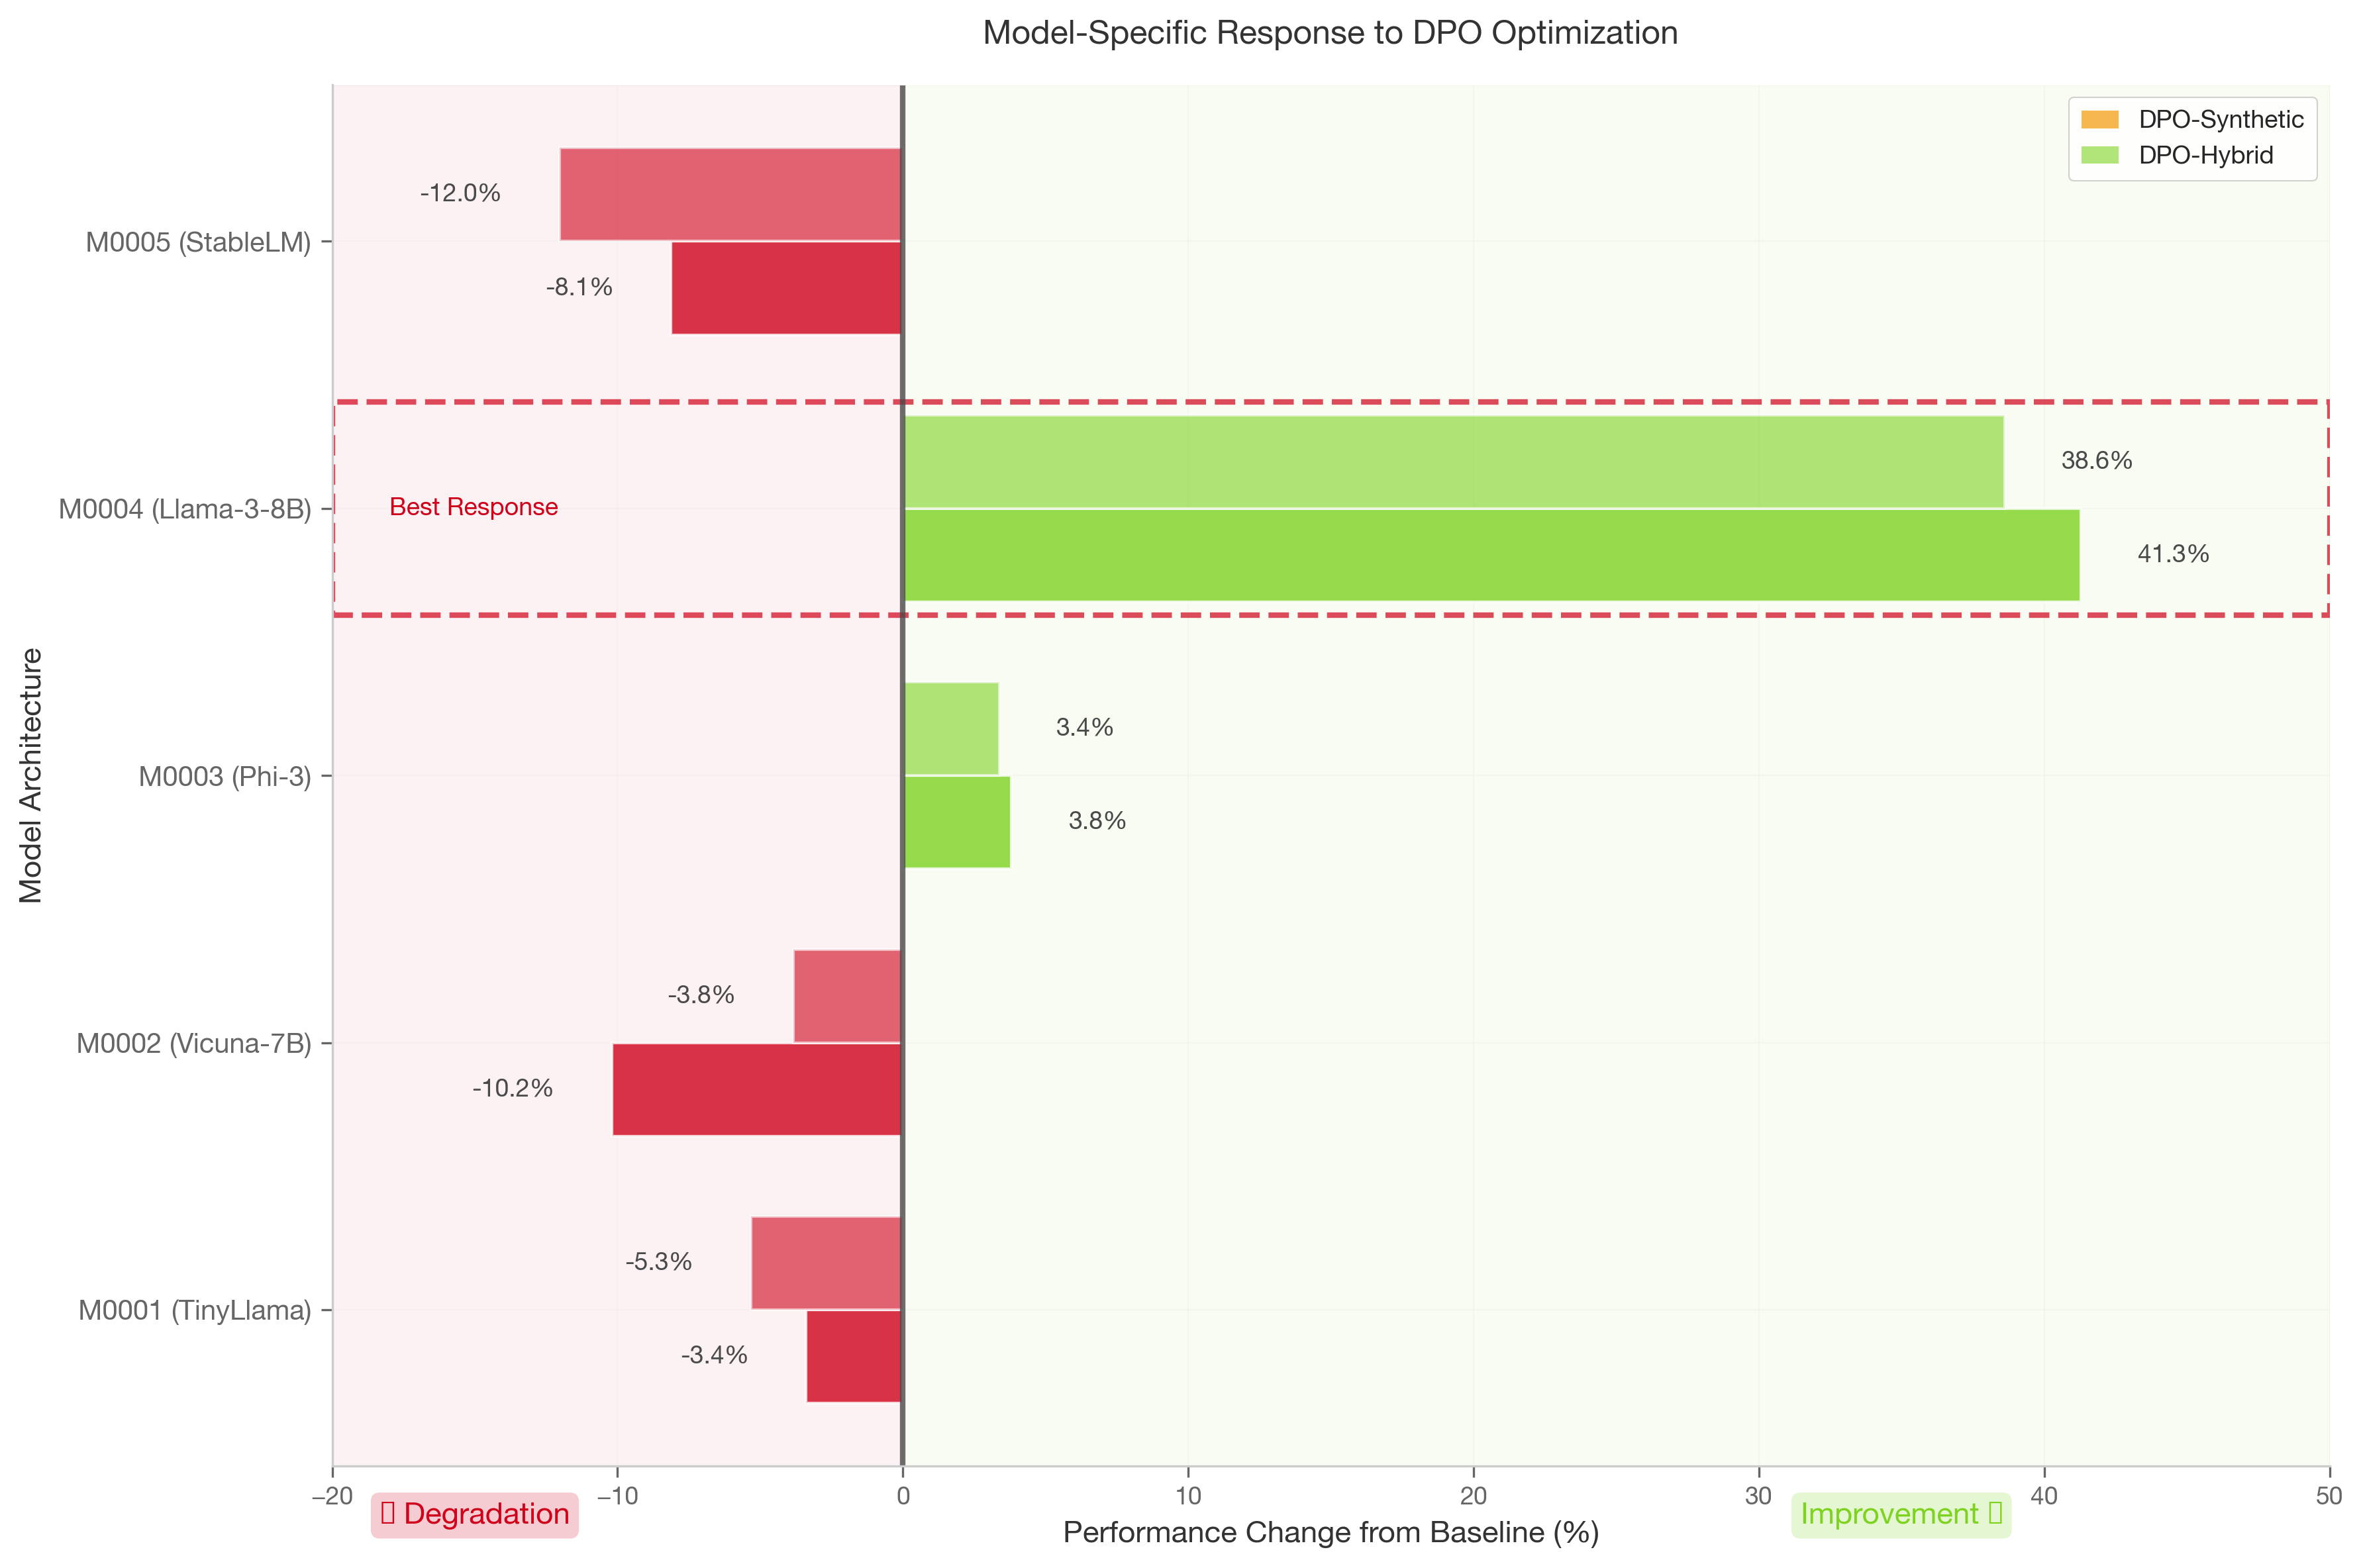
\includegraphics[width=0.8\textwidth]{figures/model_specific_improvements.png}
\caption[Model-Specific Improvement Forest Plot]{Model-Specific Improvement Forest Plot. Forest plot showing improvement rates for each individual model across DPO-Synthetic and DPO-Hybrid variants compared to baseline. Model M0004 (Llama-3-8B) demonstrates the largest improvements (+41.3\% Synthetic, +38.6\% Hybrid), while M0001 (TinyLlama), M0002 (Vicuna-7B), and M0005 (StableLM) show performance decreases. M0003 (Phi-3) shows modest improvements. Confidence intervals for improvement percentages illustrate differential optimization effectiveness across architectures.}
\label{fig:model-improvements}
\end{figure}

\begin{figure}[H]
\centering
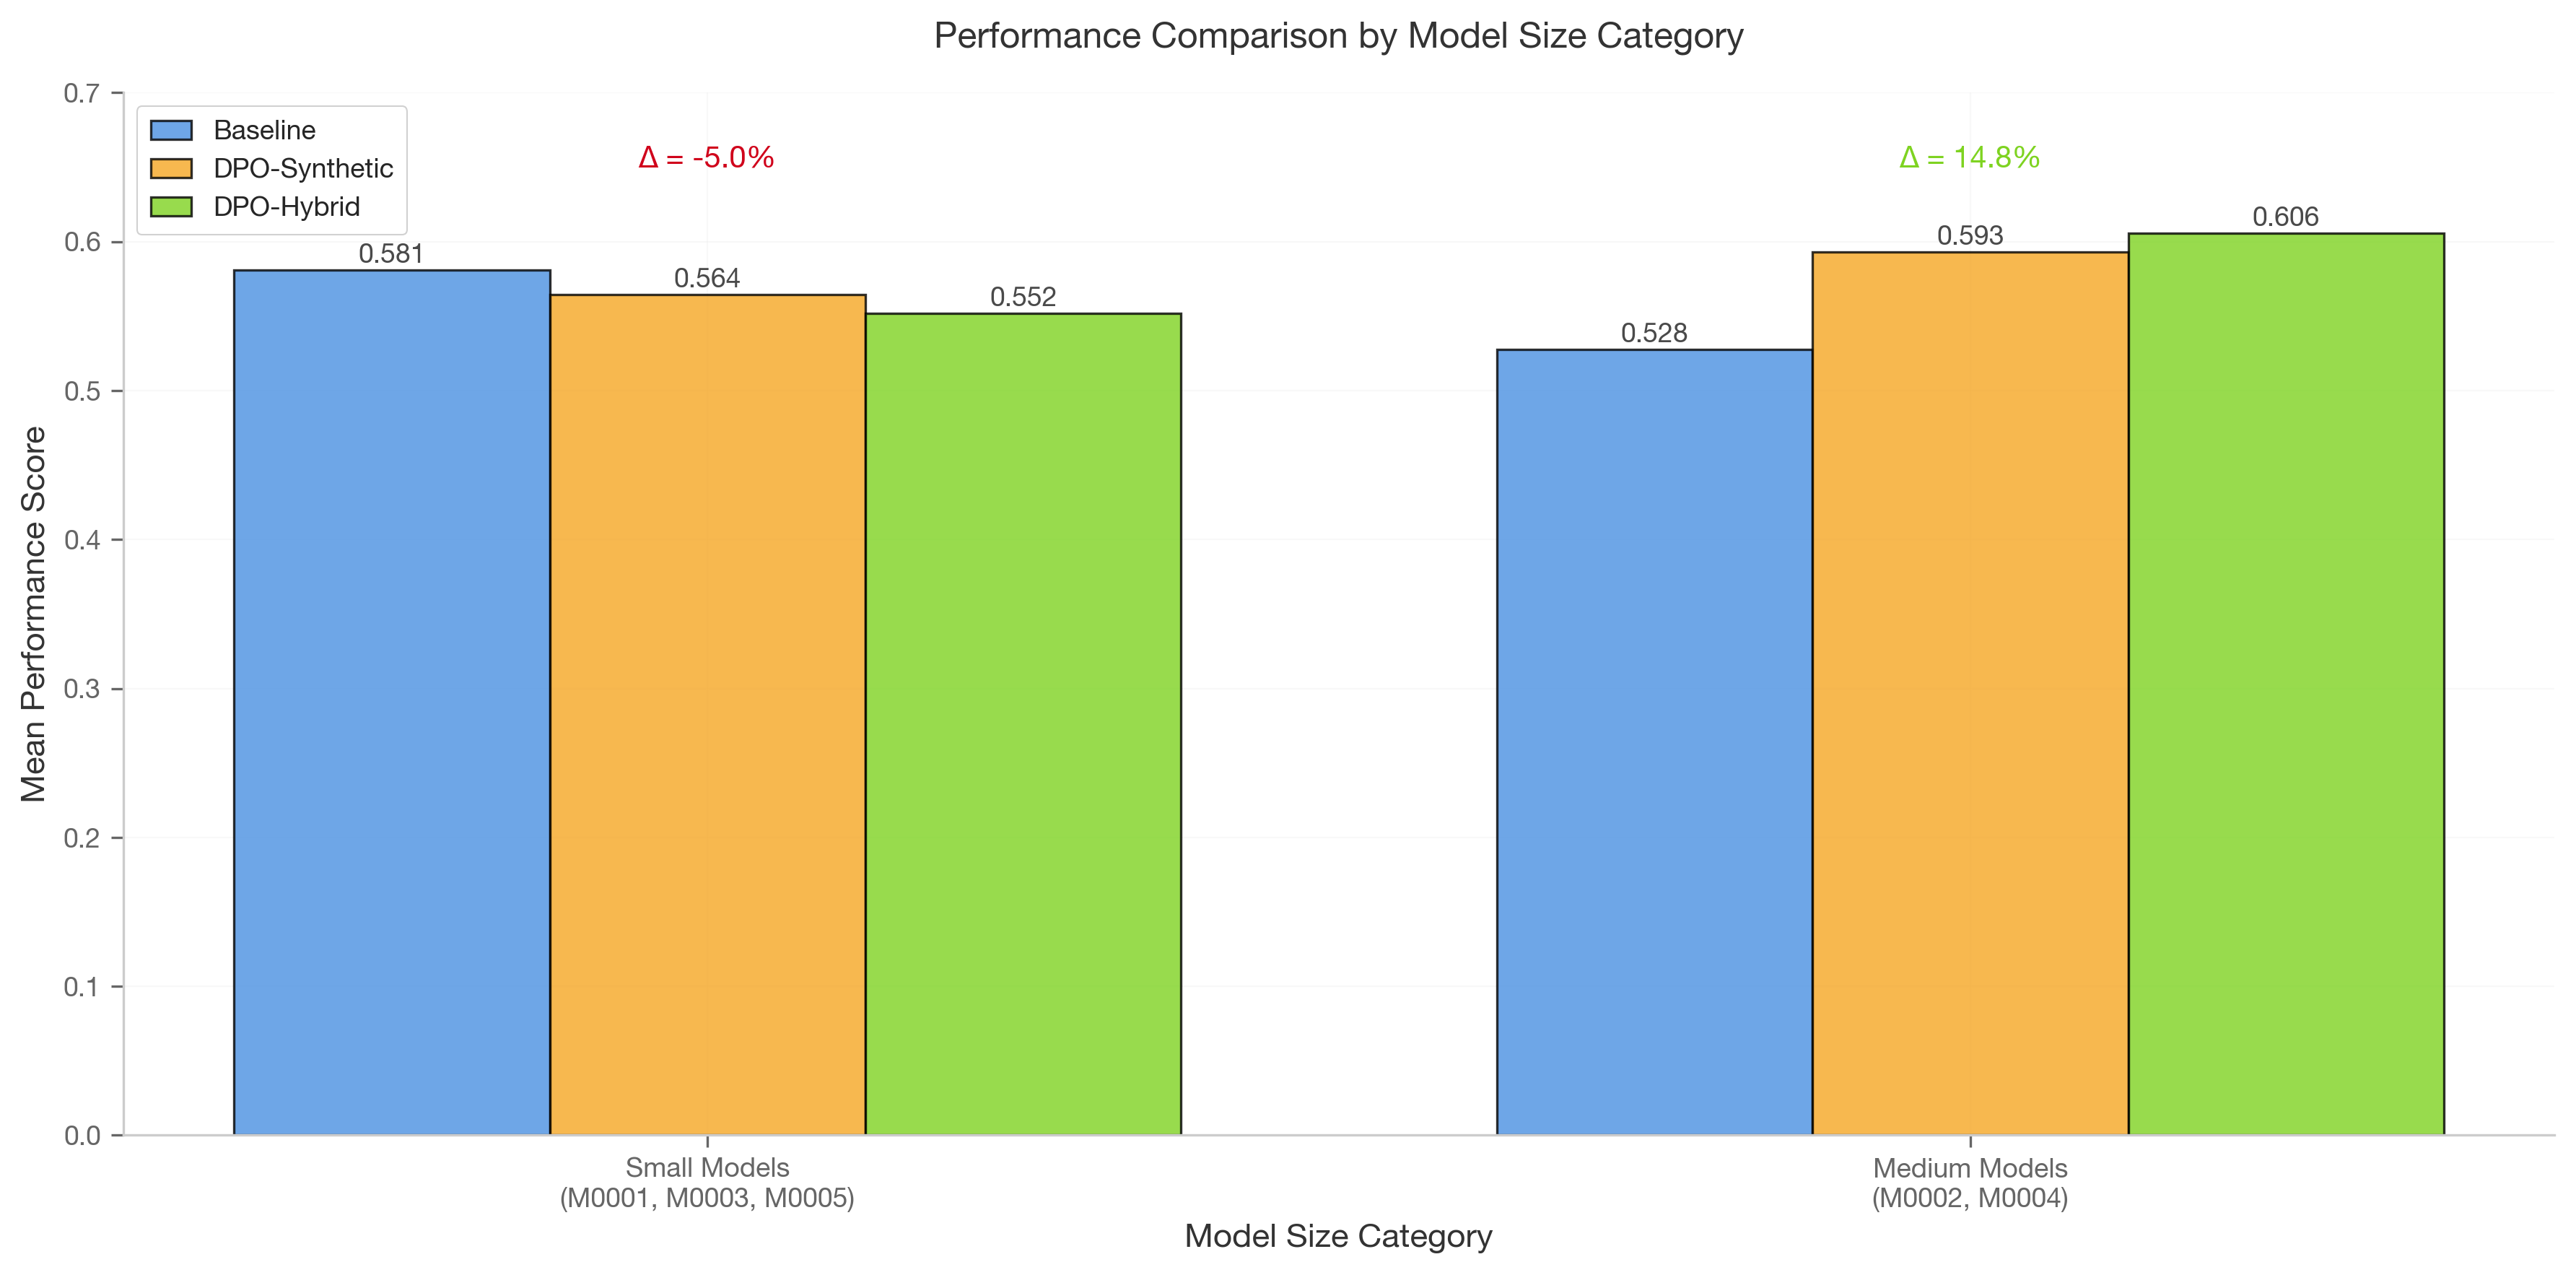
\includegraphics[width=0.8\textwidth]{figures/model_size_comparison.png}
\caption[Model Size Group Performance Comparison]{Model Size Group Performance Comparison. Performance comparison by model size groups showing aggregated performance within small models (M0001, M0003, M0005) and medium models (M0002, M0004). Small models show baseline mean = 0.581, DPO-Synthetic mean = 0.564, DPO-Hybrid mean = 0.552. Medium models show baseline mean = 0.528, DPO-Synthetic mean = 0.593, DPO-Hybrid mean = 0.606. Size-dependent responses to optimization indicate architecture-specific effectiveness patterns across different model scales.}
\label{fig:size-comparison}
\end{figure}

\section{Domain-Specific Performance Analysis}
\label{sec:category-analysis}

Performance analysis across charity topic categories (Table~\ref{tab:category-analysis}) revealed differential optimization effects depending on content domain. Environmental topics demonstrated the largest improvement with DPO-Synthetic optimization (+17.5\%), while Community/Social topics showed moderate gains (+6.0\%). Healthcare/Medical topics exhibited decreases with DPO-Synthetic (-6.9\%) but improvements with DPO-Hybrid (+4.6\%).

\begin{table}[H]
\centering
\caption{Performance by Topic Category}
\label{tab:category-analysis}
\begin{tabular}{lcccccc}
\toprule
\multirow{2}{*}{\textbf{Category}} & \multicolumn{2}{c}{\textbf{Baseline}} & \multicolumn{2}{c}{\textbf{DPO-Synthetic}} & \multicolumn{2}{c}{\textbf{DPO-Hybrid}} \\
\cmidrule(lr){2-3} \cmidrule(lr){4-5} \cmidrule(lr){6-7}
& \textbf{M} & \textbf{N} & \textbf{M} & \textbf{$\Delta\%$} & \textbf{M} & \textbf{$\Delta\%$} \\
\midrule
Healthcare/Medical & 0.597 & 60 & 0.556 & -6.9\% & 0.625 & +4.6\% \\
Education/Youth & 0.534 & 65 & 0.514 & -3.8\% & 0.543 & +1.6\% \\
Environmental & 0.543 & 60 & 0.638 & +17.5\% & 0.569 & +4.8\% \\
Community/Social & 0.565 & 65 & 0.599 & +6.0\% & 0.561 & -0.8\% \\

\bottomrule
\end{tabular}
\begin{tablenotes}
\small
\item Note: $\Delta\%$ represents percentage change from baseline. Categories represent balanced segments of the evaluation data.
\end{tablenotes}
\end{table}

Category-specific analysis revealed substantial variation in optimization effectiveness across content domains, with Environmental categories demonstrating the largest positive response to DPO-Synthetic optimization (+17.5\%). Healthcare/Medical topics showed mixed results, with DPO-Synthetic producing decreases (-6.9\%) while DPO-Hybrid resulted in performance improvements (+4.6\%). Education/Youth and Community/Social topics exhibited minimal changes across optimization variants.

The observed category-specific patterns suggest domain-dependent optimization effectiveness, with certain charitable cause types exhibiting greater susceptibility to preference-based optimization approaches. However, the overall statistical equivalence indicates these domain-specific effects were insufficient to produce detectable population-level improvements across the complete evaluation framework.


\section{Predictive Validity Assessment}
\label{sec:validation-results}

Methodology validation revealed complete failure of theoretical predictions, with all predicted effect sizes substantially overestimating actual empirical effects. The observed $\eta^2 = 0.001$ fell well below the methodology-predicted threshold of $\eta^2 > 0.06$, indicating that optimization approaches proved ineffective at achieving detectable population-level performance improvements.

\begin{table}[H]
\centering
\caption{Methodology Validation: Predicted vs Actual Results}
\label{tab:methodology-validation}
\begin{tabular}{lccccc}
\toprule
\textbf{Comparison} & \textbf{Predicted d} & \textbf{Actual d} & \textbf{Within Range} & \textbf{Validation} \\
\midrule
Baseline vs DPO-Synthetic    & 0.5--0.7 & -0.065 & \xmark & FAIL \\
Baseline vs DPO-Hybrid       & 0.7--1.0 & -0.056 & \xmark & FAIL \\
DPO-Synthetic vs DPO-Hybrid  & 0.3--0.5 & 0.011 & \xmark & FAIL \\
\midrule
ANOVA $\eta^2$ Threshold & $>0.06$ & 0.001 & \xmark & FAIL \\
Expert Correlation & $>0.80$ & N/A & N/A & N/A \\
\midrule
\textbf{Overall Status} & \multicolumn{4}{c}{\textbf{FAIL}} \\
\bottomrule
\end{tabular}
\begin{tablenotes}
\small
\item Note: Methodology validation assesses whether empirical results match theoretical predictions. All effect size predictions and ANOVA threshold failed validation.
\end{tablenotes}
\end{table}

Predictive validity assessment documented systematic failure across all theoretical predictions, with empirical effect sizes falling substantially below predicted ranges for all pairwise comparisons. The largest discrepancy occurred in the Baseline vs DPO-Hybrid comparison (predicted d = 0.7-1.0, actual d = -0.056), representing a prediction error exceeding 0.75 effect size units.

The comprehensive validation failure indicates fundamental limitations in the theoretical framework underlying optimization effectiveness predictions (Figure~\ref{fig:methodology-validation}). All optimization approaches failed to achieve predicted performance improvements, with empirical results consistently demonstrating statistical equivalence rather than the anticipated differential effectiveness patterns across optimization strategies.